% !TeX root = ./preamble.tex
\documentclass[11pt,a4paper,notitlepage]{article}

\usepackage{amsmath}							% American Mathematical Society package.
\usepackage{amsfonts}
\usepackage{amssymb}
\usepackage{bm}									% Bold math.
\usepackage[utf8]{inputenc}
\usepackage[slovene]{babel}
\usepackage[style=german]{csquotes}
\usepackage[									% BibLaTex/Biber bibliography.
	backend=biber,
	style=ieee]{biblatex}
\addbibresource{preamble.bib}
\usepackage{graphicx}							% Define font colors, page colors, boxes with background color, rotate text in a box, scale text vertically and horizontally, put graphics in a box.
\usepackage{verbatim}							% Multiline comments.
\usepackage{setspace}							% Adjust line spacing.
\usepackage{parskip}
\setlength{\parindent}{0pt}
\usepackage{fancyhdr}							% Fancy headers.
\linespread{1}
\usepackage[font=normalsize]{caption}  		 	% Captions for figures inside minipages. Allows setting alignment inside captions.
\usepackage{subcaption}
\usepackage[retainorgcmds]{IEEEtrantools}  		% Best tool for multiline equations or equation arrays.
\usepackage[unicode]{hyperref} 					% Hyperlinks ToC entries to their respective pages.
\hypersetup{
    colorlinks,
    citecolor=black,
    filecolor=black,
    linkcolor=black,
    urlcolor=black
}
\usepackage{url} 								% Allows long URLs.
\usepackage{placeins} 							% FloatBarrier.
\usepackage{booktabs}							% TabItem (manually insert list item dot).
\usepackage{xcolor}								% Required by tabu.
\usepackage{colortbl}							% Required by tabu.
\usepackage{tabu}								% Width-adjustable tabular.
\usepackage{multirow}							% Columns spanning multiple rows.
\newcommand{\tabitem}{~~\llap{\textbullet}~~}	% TabItem command.
\usepackage{wrapfig}							% Figures which text can flow around.
\usepackage{physics}

% OKRAJŠAVE MATEMATIČNIH SIMBOLOV

\def\rcurs{{\mbox{$\resizebox{.09in}{.08in}{
\includegraphics[trim= 1em 0 14em 0,clip]{TeX/ScriptR}}$}}}		% Cursive r.
\def\brcurs{{\mbox{$\resizebox{.09in}{.08in}{
\includegraphics[trim= 1em 0 14em 0,clip]{TeX/BoldR}}$}}}		% Bold cursive r.
\renewcommand{\arraystretch}{1.3} 				% Za razmik med vrsticami tabele.
\newcommand{\ud}{\mathrm{d}} 					% Krajše ime diferenciala.
\newcommand{\uD}{\mathrm{D}}					% Diferencialni operator.
\newcommand{\pd}{\partial}						% Parcialni odvod.
\newcommand{\del}{\bm{\nabla}}					% Nabla.
\newcommand{\mathbsf}[1] {\bm{\mathsf{#1}}}
\renewcommand{\Re}{\operatorname{Re}}		  	% Operator za realni del kompleksnega števila.
\renewcommand{\Im}{\operatorname{Im}} 			% Operator za imaginarni del kompleksnega števila.


% NASTAVITEV RAZMIKA MED BESEDILOM IN ENAČBO
\setlength{\belowdisplayskip}{11pt} 			% Razmik pod enačbo, ko je vrstica polna.
\setlength{\abovedisplayskip}{11pt} 			% Razmik nad enačbo, ko je vrstica polna.
\setlength{\belowdisplayshortskip}{11pt}  		% Razmik pod enačbo, ko vrstica ni polna.
\setlength{\abovedisplayshortskip}{0pt}   		% Razmik nad enačbo, ko vrstica ni polna.

\pagestyle{fancy}	% Setting for FancyHdr package. Must occur before length adjustments.

% FIRST PAGE LAYOUT / VERTICAL LENGTHS
\setlength{\voffset}{-1.0in}					% Top to Header Top Margin = 1 inch+\voffset
\setlength{\topmargin}{1.0cm}					% Header Top Margin Height
\setlength{\headheight}{1.75cm}
\setlength{\headsep}{0.35cm}					% Header Lower Margin Height
\setlength{\textheight}{24.7cm}					% Header Lower Margin to Footer height
\setlength{\footskip}{1.0cm}
% FIRST PAGE LAYOUT / HORIZONTAL LENGTHS
\setlength{\headwidth}{17.0cm}
\setlength{\hoffset}{-1.0in}					% Left page padding = 1 inch + \hoffset
\setlength{\oddsidemargin}{2.0cm}
\setlength{\textwidth}{17.0cm}
\setlength{\marginparsep}{0.0cm}
\setlength{\marginparwidth}{0.0cm}				% Width of "side notes margin."

\fancyhead[L]{
	\large{Marko Petek} \\[0.3cm]
}
\fancyhead[C]{
\includegraphics[height=1.6cm]{Slike/logo-um-fnm}}
\fancyhead[R]{									% Right header = Place and date.
	\large{Maribor, 19.\ I.\ 2019} \\[0.3cm]
}
\cfoot{\thepage}								% Footer center = page number.			
\renewcommand{\headrulewidth}{0.0cm}			% Horizontal line in header. 0 = no horizontal line.
\renewcommand{\footrulewidth}{0.0cm}			% Horizontal line in footer

\begin{document}
	\begin{center}
	\textbf{\LARGE{Metoda končnih elementov, ki minimizira kvadrat ostanka aproksimacije (\texttt{LSFEM})}}\\[0.25cm]
	\large{Seminarska naloga pri Naprednih numeričnih metodah}\\[0.7cm]
\end{center}

Numerično reševanje parcialnih diferencialnih enačb (\texttt{PDE}) je zaradi pomanjkanja vsestranskega algoritma še zmeraj bolj umetnost kot ustaljena znanost \cite{JiangB-LSFEM}. Pri zapletenih problemih hitro prispemo do vznožja gore matematične teorije, ki je ni moč zaobiti. Zaradi množice različnih pristopov reševanja ter raztresene in neprijazno napisane literature, lahko le ugibamo, kako visoko se bomo na poti do prelaza morali povzpeti. Zapletenim problemom prostorske dinamike v:
\begin{center}
	\begin{tabular}[h]{lll}
		\tabitem dinamiki tekočin,\hspace{1cm}	&	\tabitem termodinamiki,\hspace{2.5cm}	&	\tabitem elektrodinamiki,\\
		\tabitem kvantni teoriji,	&	\tabitem splošni teoriji relativnosti,&	\\
	\end{tabular}
\end{center}
kjer naletimo na \texttt{PDE}, se tako tudi v višjem izobraževanju najraje izognemo. Metoda končnih elementov (\texttt{FEM}), ki minimizira kvadrat ostanka aproksimacije (\texttt{LSFEM} = Least Squares \texttt{FEM}), obeta razvoj vsestranskega algoritma za reševanje \texttt{PDE} in s tem približanje omenjenih problemov širšemu krogu raziskovalcev.
	% !TeX root = ./seminar.tex
\section{Podlaga za temelje \texttt{LSFEM}}

Kadar obravnavamo prostorsko dinamiko (npr.\ tok tekočine), lahko fizični prostor modeliramo kot 1, 2 ali 3-mnogoterost. Teorijo \texttt{LSFEM} bomo predstavili na splošnem primeru $d$-mnogoterosti, za ponazoritev pa na njih sproti gradili konkretni 2D primer.

\begin{wrapfigure}{r}{6cm}
	\vspace{-3mm}
	\centering
	\captionsetup{type=figure}
	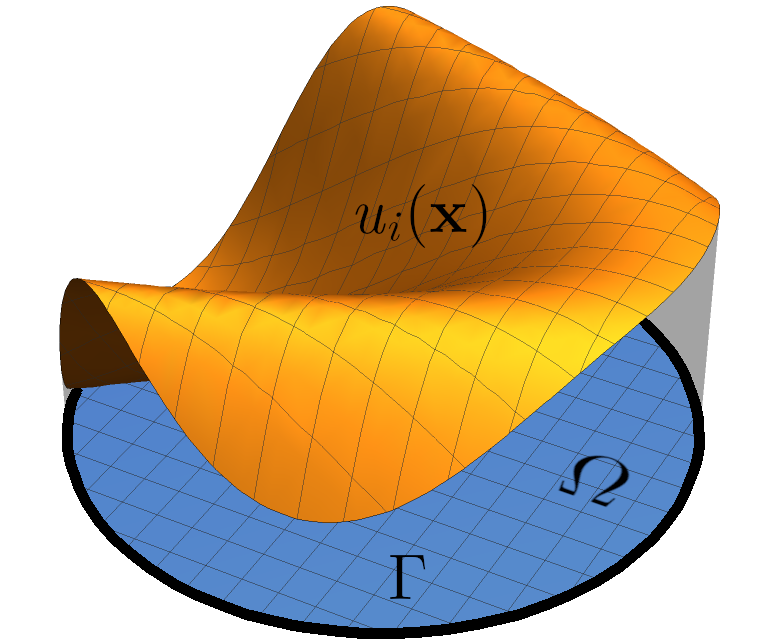
\includegraphics[width=5.5cm]{Slike/funkcijaInDomenaG}
	\caption{Domena $\Omega$, meja domene $\Gamma$ in komponenta rešitve $u_i(\mathbf{x})$.}
\label{fig:funkInDom}
\vspace{0.2cm}
\end{wrapfigure}

Naj bo torej prizorišče dogajanja $d$-mnogoterost $\Omega$ (slika \ref{fig:funkInDom}), opremljena s krajevnim vektorjem:
\vspace{-1.5mm}
\begin{equation}
\mathbf{x} = \{x_1, ..., x_d\} \ . \nonumber
\vspace{-1mm}
\end{equation}
Pri reševanju sistema $m$ \texttt{PDE} iščemo nabor funkcij:
\vspace{-0.5mm}
\begin{equation}
	\mathbf{u}(\mathbf{x}) =  \{u_1(\mathbf{x}), ..., u_m(\mathbf{x})\} \ , \nonumber
	\vspace{-1mm}
\end{equation}
ki v vsaki točki domene $\Omega$ zadosti sistemu \texttt{PDE}, na meji $\Gamma$ pa robnim pogojem. Konkretni primer bomo gradili na 2D primeru s štirimi spremenljivkami, pri katerem bosta krajevni vektor in vektor odvisnih spremenljivk enaka:
\vspace{2.5mm}
\begin{equation}
	\hspace{-60mm} \mathbf{x} = \{x, y\} \quad \text{in} \quad \mathbf{u} =  \{u, v, p, \omega\} \ . \nonumber
\end{equation}
\\[-4mm]
Dinamiko naj opiše \textbf{sistem Stokesovih enačb} za nestisljive tekočine v obliki hitrost-tlak-vrtinčnost, ki jim v prid nazornosti primera umetno dodamo koeficiente $\alpha(\mathbf{x})$, $\beta(\mathbf{x})$, $\gamma(\mathbf{x})$ in $\delta(\mathbf{x})$:\\[0.05cm]
\begin{minipage}{0.11\textwidth}
	\hspace{1cm}
\end{minipage}
\begin{minipage}{0.33\textwidth}
\begin{IEEEeqnarray}{rl}
	\alpha \mkern2mu \frac{\pd p}{\pd x} + \beta \mkern2mu \frac{\pd \omega}{\pd y} & \ = \, f_x \ ,
	\label{eq:StokesXMom}
	\\[0.3cm]
	\gamma \mkern2mu \frac{\pd p}{\pd y} - \delta \mkern2mu \frac{\pd \omega}{\pd x} & \ = \, f_y \ ,
\end{IEEEeqnarray}
\end{minipage}
\begin{minipage}{0.33\textwidth}
\begin{IEEEeqnarray}{rl}
	\frac{\pd u}{\pd x} + \frac{\pd v}{\pd y} & \ = \, 0 \ , \label{eq:StokesDiv}
	\\[0.3cm]
	\omega + \frac{\pd u}{\pd y} - \frac{\pd v}{\pd x} & \ = \, 0 \ .
	\label{eq:StokesCurl}
\end{IEEEeqnarray}
\end{minipage}\\[0.4cm]
Stokesove enačbe ustrezajo stacionarnim Navier-Stokesovim enačbam brez nelinearnih konvektivnih členov, ki jih moramo pri numeričnem reševanju linearizirati. Ker ta korak za ponazoritev \texttt{LSFEM} ni ključen, se mu na tak način izognemo. Stokesove enačbe opisujejo plazeče se tokove, pri katerih je konvekcija gibalne količine (zaradi gibanja) majhna v primerjavi z njeno difuzijo (zaradi viskoznosti).

\setlength{\textheight}{26.4cm}
\pagebreak
\setlength{\topmargin}{1.6cm}			% Header Top Margin Height
\setlength{\headheight}{0.0cm}
\setlength{\headsep}{0.0cm}			% Header Lower Margin Height	 Footer height
\fancyhf{}
\fancyfoot[C]{\thepage}

V enačbah ni časovnih odvisnosti (razen preko časovno odvisnih robnih pogojev), zato so takšni tokovi časovno obrnljivi: časovno obrnjena rešitev enačb je prav tako rešitev (slika \ref{fig:TaylorCouette}).

\begin{figure}[!ht]
	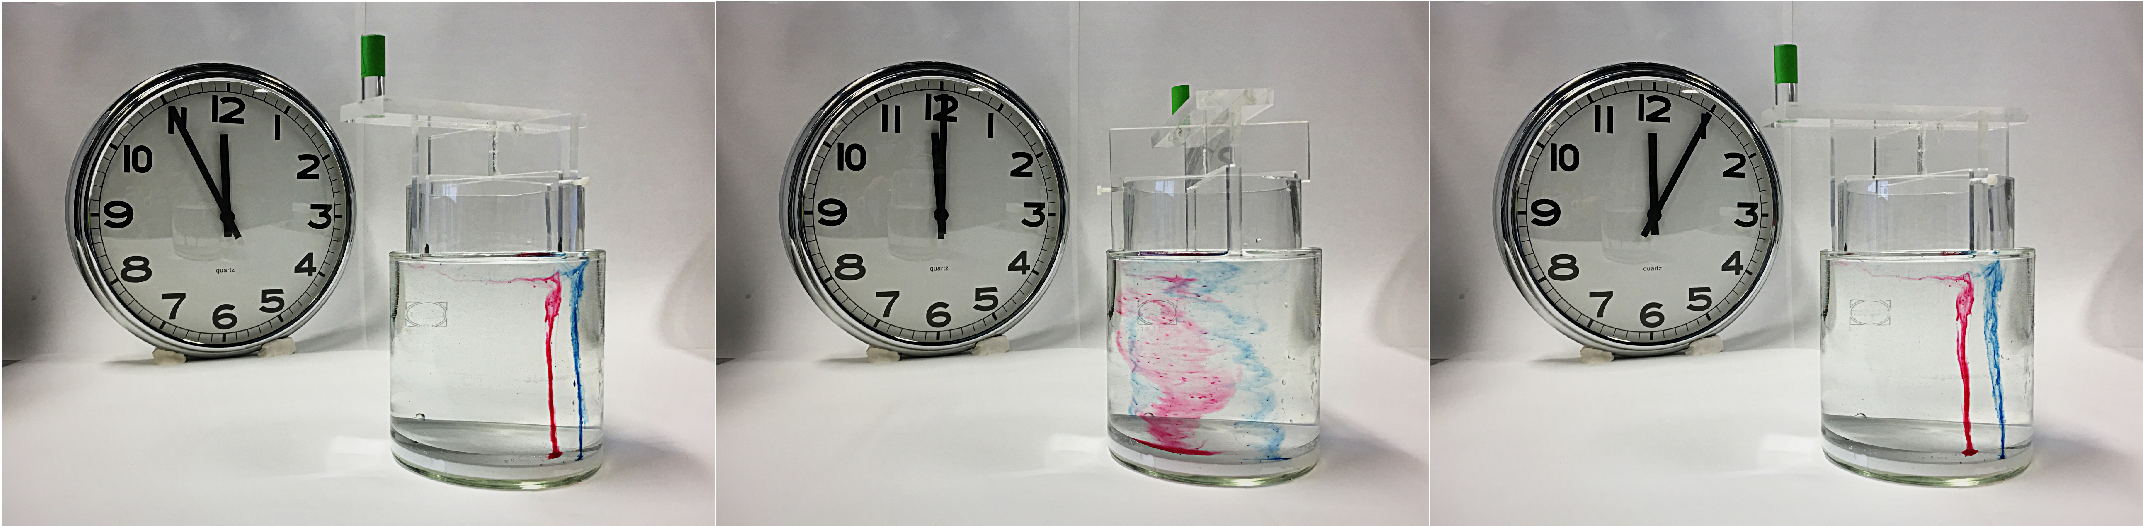
\includegraphics[width = 1\textwidth]{Slike/TaylorCouette}
	\caption{Zabaven eksperiment, pri katerem se v ozkem prostoru med dvema koncentričnima valjema nahaja viskozna tekočina, ki jo na dveh mestih označimo z liso barvila. Valja pet minut vrtimo v nasprotnih smereh (Stokesov tok, ki tako nastane, imenujemo Taylor-Couettov tok), da se lisi pomešata, nato smeri vrtenja obrnemo in po petih minutah se lisi ponovno sestavita. Pridobljeno iz  \cite{Wiki-StokesFlow}.}
	\label{fig:TaylorCouette}
\end{figure}

Sistem \texttt{PDE}, ki ga obravnavamo, zapišemo bolj jedrnato v matrični obliki. To je enostavno, če je sistem linearen. Uvedemo diferencialni operator $\mathbsf{A}$:
\begin{equation}
	\mathbsf{A}(\mathbf{x}) \mkern2mu
	=
	\, \mathbsf{A}_0(\mathbf{x}) + \mathbsf{A}_1(\mathbf{x}) \frac{\pd}{\pd x_1} + \, \mathbsf{A}_2(\mathbf{x}) \frac{\pd}{\pd x_2} \ ,
	\label{eq:AMatrixDefinition}
	\vspace{-1mm}
\end{equation}
\vspace{1mm}
s katerim lahko sistem enačb zapišemo kot:
\begin{equation}
	\qty(\mathbsf{A}_0(\mathbf{x}) + \mathbsf{A}_1(\mathbf{x}) \mkern1mu \frac{\pd}{\pd x_1} + \mathbsf{A}_2(\mathbf{x}) \mkern1mu \frac{\pd}{\pd x_2}) \mkern-1mu \cdot \mkern-1mu \mathbf{u}(\mathbf{x}) \, = \, \mathbf{f}(\mathbf{x}) \ ,
	\label{eq:matrixPDE1}
	\vspace{-1mm}
\end{equation}
oziroma na kratko:
\vspace{2mm}
\begin{equation}
	\hspace{12mm} \boxed{
		\, \vphantom{\big(} \mathbsf{A}(\mathbf{x}) \mkern-1.5mu \cdot \mkern-1.5mu \mathbf{u}(\mathbf{x}) = \, \mathbf{f}(\mathbf{x}) \,
	}\hspace{1.3cm} \texttt{sistem PDE .}
	\label{eq:compactPDE}
	\vspace{1.5mm}
\end{equation}
V matriko $\mathbsf{A}_0$ spravimo vse koeficiente pred členi z odvisnimi spremenljivkami, v matriko $\mathbsf{A}_1$ vse koeficiente pred členi z odvodi odvisnih spremenljivk po koordinati $x_1$ in v $\mathbsf{A}_2$ vse koeficiente pred členi z odvodi odvisnih spremenljivk koordinati $x_2$. Ostale člene zložimo v vektor $\mathbf{f}$. Enačbe \eqref{eq:StokesXMom} - \eqref{eq:StokesCurl} lahko v duhu enačbe \eqref{eq:matrixPDE1} zapišemo kot:
\vspace{1.5mm}
\begin{equation*}
	\left[ \,
	\begin{pmatrix}
		0 & 0 & 0 & 0 \\
		0 & 0 & 0 & 0 \\
		0 & 0 & 0 & 0 \\
		0 & 0 & 0 & 1
	\end{pmatrix} +
	\begin{pmatrix}
		0 & 0 & \alpha & 0 \\
		0 & 0 & 0 & -\delta \\
		1 & 0 & 0 & 0 \\
		0 & -1 & 0 & 0
	\end{pmatrix} \frac{\pd}{\pd x} +
	\begin{pmatrix}
		0 & 0 & 0 & \beta \\
		0 & 0 & \gamma & 0 \\
		0 & 1 & 0 & 0 \\
		1 & 0 & 0 & 0 \\
	\end{pmatrix} \frac{\pd}{\pd y} \, \right]
	\mkern0mu \cdot \mkern2mu
	\begin{pmatrix}
		u \\ v \\ p \\ \omega
	\end{pmatrix}
	\ = \
	\begin{pmatrix}
		f_x(\mathbf{x}) \\ f_y(\mathbf{x}) \\ 0 \\ 0
	\end{pmatrix} \ .
	\vspace{1mm}
\end{equation*}
	\section{Temelji \texttt{LSFEM}}

Vse različice \texttt{FEM} vsaj okvirno temeljijo na variacijskem pristopu, kjer ne operiramo neposredno na \texttt{PDE}, ampak jih najprej pretvorimo v enakovreden variacijski problem: omislimo si \textbf{poskusno funkcijo} $\mathbf{w}(\mathbf{x})$, ki jo napnemo nad domeno $\Omega$, in izberemo funkcional $I[\mathbf{w}(\mathbf{x})]$, ki za vsako $\mathbf{w}(\mathbf{x})$ vrne neko realno število. Za uspešnost variacijskega pristopa moramo izbrati funkcional, ki vrne najmanjšo vrednost, ko je $\mathbf{w}(\mathbf{x})$ enaka rešitvi. Kadar obstaja s sistemom \texttt{PDE} povezan energijski potencial, je le-ta fizikalno najintuitivnejša izbira za konstrukcijo funkcionala. Zato ni presenetljivo, da je bila \textbf{Rayleigh-Ritzeva različica} \texttt{FEM} (\texttt{RRFEM}), ki jo na tak način dobimo, razvita prva \cite{RitzW-Variationsprobleme}. Konstrukcija funkcionala in njegova minimizacija sta tipična koraka variacijskega pristopa in nista specifična za \texttt{RRFEM}: vzamemo neko funkcijo poskusne funkcije $F\left(\mathbf{w}\right)$ in jo integriramo po domeni $\Omega$:
\vspace{-1mm}
\begin{equation}
	\hspace{17mm}
	\boxed{
		\vphantom{\bigg(} \ I\big[\mathbf{w(x)}\big]\mkern2mu
		=
		\int_{\Omega} \mkern-4mu F\big(\mathbf{w(x)}\big) \mkern5mu \ud \Omega \ 
	}
	\hspace{13mm} \texttt{funkcional poskusne funkcije} \ .
	\label{eq:GeneralFunctional}
\end{equation}
Ko smo prepričani, da ima funkcional \eqref{eq:GeneralFunctional} minimum pri rešitvi $\mathbf{u}(\mathbf{x})$, sledimo znanemu Euler-Lagrange\-ve\-mu postopku. Ta nas pripelje do variacijske izjave, ki velja le, kadar je poskusna funkcija $\mathbf{w}(\mathbf{x})$ enaka rešitvi $\mathbf{u}(\mathbf{x})$. Poskusno funkcijo razvijemo okoli rešitve:
\begin{equation}
	\widetilde{\mathbf{w}}(\mathbf{x}, \varepsilon) \mkern2mu
	=
	\, \mathbf{u}(\mathbf{x}) \mkern1mu + \mkern1.5mu \varepsilon \mathbf{v}(\mathbf{x}) \ ,
	\label{eq:trialFuncAroundSol}
\end{equation}
kjer je $\mathbf{v}(\mathbf{x})$ poljubna odmična funkcija, $\varepsilon$ pa realno število. Kadar gre $\varepsilon$ proti nič, gre $\widetilde{\mathbf{w}}(\mathbf{x}, \varepsilon)$ proti rešitvi problema $\mathbf{u}(\mathbf{x})$, hkrati pa vemo, da ima funkcional $I$ pri $\mathbf{u}(\mathbf{x})$ minimum. Minimum funkcionala poiščemo tako, da razvoj \eqref{eq:trialFuncAroundSol} vstavimo v funkcional \eqref{eq:GeneralFunctional} namesto $\mathbf{w}(\mathbf{x})$ in izraz odvajamo po $\varepsilon$:
\begin{equation*}
	\frac{\ud I}{\ud \varepsilon} \,
	=
	\, \int_{\Omega} \frac{\ud}{\ud \varepsilon} F(\widetilde{\mathbf{w}}) \, \ud \Omega \,
	=
	\, \int_{\Omega} \left(\frac{\ud F}{\ud \widetilde{\mathbf{w}}}\right)^\mathsf{\mkern-7mu T} \mkern-5mu \cdot \mkern-1mu \frac{\ud \widetilde{\mathbf{w}}}{\ud \varepsilon} \ \ud \Omega \,
	=
	\, \int_{\Omega} \left(\frac{\ud F}{\ud \widetilde{\mathbf{w}}}\right)^\mathsf{\mkern-7mu T} \mkern-5mu \cdot \mkern-1mu \mathbf{v} \ \ud \Omega \ ,
\label{eq:funcDerivative}
\end{equation*}
nato pa $\varepsilon$ v \eqref{eq:funcDerivative} pošljemo proti nič in celoten izraz enačimo z nič:
\begin{equation*}
	\lim_{\varepsilon \rightarrow 0} \frac{\ud I}{\ud \varepsilon} \,
	=
	\, \lim_{\varepsilon \rightarrow 0} \int_{\Omega} \left(\frac{\ud F\big(\widetilde{\mathbf{w}}(\mathbf{x}, \varepsilon)\big)}{\ud \widetilde{\mathbf{w}}}\right)^\mathsf{\mkern-7mu T} \mkern-5mu \cdot \mathbf{v(\mathbf{x})} \ \ud \Omega \,
	=
	\, 0 \ .
\end{equation*}
Limita deluje le na prvi člen v integrandu, zato se variacijska izjava glasi:
\begin{equation}
	\boxed{\, \vphantom{\bigg)^2_3}
		\int_{\Omega} \, \lim_{\varepsilon \rightarrow 0} \left(\frac{\ud F(\widetilde{\mathbf{w}})}{\ud \widetilde{\mathbf{w}}} \right)^\mathsf{\mkern-7mu T} \mkern-5mu \cdot \mkern-1mu \mathbf{v} \ \ud \Omega \, = \, 0 \ , \quad \forall \mathbf{v(\mathbf{x})}\,
	}
	\hspace{1.3cm} \texttt{variacijska izjava} \ .
	\label{eq:variationalStatement}
\end{equation}
V jeziku funkcionalne analize, kjer na funkcije gledamo kot na vektorje, izjava pove naslednje: projekcija izraza v oklepaju na katerokoli odmično funkcijo $\mathbf{v(x)}$ mora biti enaka nič, ali krajše: izraz mora biti ortogonalen na katerokoli $\mathbf{v(x)}$.

$F\left(\mathbf{w}(\mathbf{x})\right)$ v funkcionalu poskusne funkcije je pri \texttt{RRFEM} energijski potencial, funkcional pa torej skupna potencialna energija sistema, ki jo rešitev $\mathbf{u}(\mathbf{x})$ minimizira. Zaradi tega ima \texttt{RRFEM} last\-nost najboljšega približka, diskretizacija pa vodi do simetričnega in pozitivno-definitnega sistema algebrajskih enačb, ki je zelo prikladen za reševanje s hitrimi iteracijskimi metodami. Različica metode se je izkazala v gradbenem inženirstvu, kjer je s problemom vedno povezan energijski potencial. Večina računalniških programov s tega področja zato še danes temelji na \texttt{RRFEM}.

Žal energijski potencial povezan s sistemom \texttt{PDE} ne obstaja vedno, kar je značilno za sisteme \texttt{PDE} v dinamiki tekočin. To je motiviralo razvoj Galerkinove različice \texttt{FEM} (\texttt{GFEM}), ki je zastavljena kot posplošitev \texttt{RRFEM}, vendar na precej neroden način. Ideja \texttt{GFEM} je, da lahko za vsak sistem \texttt{PDE} \eqref{eq:compactPDE} in za poljubno poskusno funkcijo $\mathbf{w(x)}$ definiramo vektor ostanka $\mathbf{R(w(x))}$. Vse člene v jedrnatem zapisu sistema \texttt{PDE} \eqref{eq:compactPDE} damo na eno stran in namesto $\mathbf{u(x)}$ pišemo $\mathbf{w(x)}$:
\begin{equation}
	\hspace{10mm} \boxed{\, \vphantom{\big(}
		\mathbf{R\big(w(x)\big)} \, = \, \mathbsf{A}(\mathbf{x}) \mkern-2.5mu \cdot \mkern-2mu \mathbf{w(x)} - \mathbf{f(x)} \,
	}\hspace{20mm} \texttt{vektor ostanka .}
	\label{eq:residual}
\end{equation}
Funkcija $\mathbf{w(x)}$, za katero je ostanek $\mathbf{R(w(x))}$ enak nič, je rešitev problema $\mathbf{u(x)}$. Idejo za izničenje ostanka vzamemo iz variacijske izjave \eqref{eq:variationalStatement}: naj bo ostanek $\mathbf{R(w(x))}$ ortogonalen na katerokoli odmično funkcijo $\mathbf{v(x)}$:
\begin{equation}
	\hspace{21mm} \int_{\Omega} \mathbf{R\big(w(x)\big)}^\mathsf{\mkern-1mu T} \mkern-4.5mu \cdot \mkern-1mu \mathbf{v(x)} \ \ud \Omega \, = \, 0 \hspace{13mm} \texttt{načelo metode uteženih ostankov .}
	\label{eq:GfemStatement}
\end{equation}
Pristop se imenuje \textbf{metoda uteženih ostankov} in nas za sebi-adjungirane ter pozitivno-definitne $\mathbsf{A}\mathbf{(x)}$ pripelje do istega sistema algebrajskih enačb kot \texttt{RRFEM}. Uporabimo pa ga lahko tudi za sisteme \texttt{PDE}, ki ne posedujejo teh lastnosti, zato daje vtis posplošitve \texttt{RRFEM}. Akademiki so pričakovali, da bo \texttt{GFEM} v dinamiki tekočin enako uspešna, kot je bila \texttt{RRFEM} v gradbenem inženirstvu, a se to ni zgodilo \cite{JiangB-LSFEM}. Ko $\mathbsf{A}$ ni sebi-adjungiran, namreč načelo \eqref{eq:GfemStatement} ni nujno zvesto osnovnemu problemu \texttt{PDE}. Metoda v tem primeru ne poseduje lastnosti najboljšega približka in v rešitvi se pogostokrat pojavijo lažne oscilacije (\emph{wiggles}). Teh se je mogoče znebiti le s hudimi izboljšavami mreže, kar očitno okrnjuje praktičnost metode. Metoda končnih diferenc in metoda končnih volumnov sta zato v dinamiki tekočin še vedno v modi.

Podobno kot pri \texttt{GFEM} se tudi pri \texttt{LSFEM} opremo na vektor ostanka \eqref{eq:residual}, a reševanja variacijskega problema se lotimo na legitimen način. Ne zanašamo se na ad hoc načela, kot je zahteva \eqref{eq:GfemStatement}, ampak začnemo od začetka - s konstrukcijo funkcionala \eqref{eq:GeneralFunctional}. Sestavimo ga s kvadratom ostanka:
\begin{equation}
	F\big(\mathbf{w(x)}\big)
	=
	\mathbf{R\big(w(x)\big)}^\mathsf{\mkern-1mu T} \mkern-5mu \cdot \mkern-1mu \mathbf{R\big(w(x)\big)} \hspace{1.3cm} \texttt{kvadrat vektorja ostanka ,}
	\label{eq:squareOfResidual}
\end{equation}
in tako se funkcional, ki ga minimiziramo, glasi:
\begin{equation}
	\boxed{
		\, I\big[\mathbf{w(x)}\big]
		=
		\int_{\Omega} \mathbf{R\big(w(x)\big)}^\mathsf{\mkern-2mu T} \mkern-5mu \cdot \mkern-1mu \mathbf{R\big(w(x)\big)} \ \ud \Omega \,
	}
	\hspace{1.3cm} \texttt{funkcional LSFEM ,}
\end{equation}
od koder dobi metoda svoje ime. Želimo dobiti variacijsko izjavo za ta specifični funkcional, zato v splošno izjavo \eqref{eq:variationalStatement} vstavimo kvadrat vektorja ostanka \eqref{eq:squareOfResidual} in postopek izpeljemo do konca. Najprej torej izračunamo odvod integranda:
\begin{equation*}
	\hspace{-10mm}
	\left(\frac{\ud F(\widetilde{\mathbf{w}})}{\ud \widetilde{\mathbf{w}}}\right)^\mathsf{\mkern-7mu T}
	\mkern1mu = \,
	\left(\frac{\ud \! \left(\mathbf{R(\widetilde{w})}^\mathsf{\mkern-1mu T} \mkern-5mu \cdot \mkern-1mu \mathbf{R(\widetilde{w})}\right)}{\ud \mathbf{\widetilde{w}}}\right)^\mathsf{\mkern-10mu T}
	= \mkern3mu
	2 \mathbf{R(\widetilde{w})}^\mathsf{\mkern-1mu T} \mkern-4mu \cdot \mkern-1mu \frac{\ud \mathbf{R(\widetilde{w})}}{\ud \mathbf{\widetilde{w}}}
	\, = \mkern5mu
	2 \mkern1mu (\mathbsf{A} \! \cdot \! \mathbf{\widetilde{w}} - \mathbf{f})^\mathsf{T} \mkern-5mu \cdot \mkern-2mu \mathbsf{A}
\end{equation*}
ter nato limito, ko gre $\varepsilon$ proti nič:
\begin{equation*}
	\hspace{-7mm}
	\lim_{\varepsilon \rightarrow 0} \left(\frac{\ud F(\widetilde{\mathbf{w}})}{\ud \widetilde{\mathbf{w}}}\right)^\mathsf{\mkern-7mu T}
	=
	\mkern5mu \lim_{\varepsilon \rightarrow 0} \ 2 \mkern1mu \big(\mathbsf{A} \! \cdot \! (\mathbf{u} \mkern-2mu + \mkern-2mu \varepsilon \mathbf{v}) - \mathbf{f}\big)^\mathsf{\mkern-2mu T} \mkern-6mu \cdot \mkern-2mu \mathbsf{A}\,
	=
	\mkern5mu 2 \mkern1mu (\mathbsf{A} \! \cdot \! \mathbf{u} - \mathbf{f})^\mathsf{T} \mkern-4mu \cdot \mkern-2mu \mathbsf{A} \ .
\end{equation*}
Variacijska izjava za minimizacijo funkcionala \texttt{LSFEM} se zato glasi:
\begin{equation*}
	\int_{\Omega} 2 \mkern1mu (\mathbsf{A} \! \cdot \! \mathbf{u} - \mathbf{f})^\mathsf{T} \mkern-4.5mu \cdot \mkern-1mu (\mathbsf{A} \! \cdot \! \mathbf{v}) \ \ud \Omega \, = \, 0 \ , \quad \forall \mathbf{v(\mathbf{x})} \ . \vphantom{\Biggr{)}}
\end{equation*}
Celoten izraz transponiramo (zamenjamo vrstni red členov v zunanjem skalarnem produktu, s čemer rezultata ne spremenimo) ter delimo z dve:
\begin{equation}
	\boxed{\
		\int_{\Omega} \, (\mathbsf{A} \! \cdot \! \mathbf{v})^\mathsf{\mkern-1mu T} \mkern-4.5mu \cdot \mkern-1mu (\mathbsf{A} \! \cdot \! \mathbf{u} - \mathbf{f}) \ \ud \Omega \, = \,
		0 \ , \hspace{5mm} \forall \mathbf{v} \vphantom{\bigg{)}} \
	}
	\hspace{10mm} \texttt{variacijska izjava LSFEM .}
	\label{eq:LsfemVariationalStatement}
\end{equation}
Izjava pravzaprav ustreza Galerkinovi formulaciji \eqref{eq:GfemStatement}, kjer namesto odmičnih funkcij samih ($\mathbf{v}$) uporabimo njihove odvode ($\mathbsf{A} \! \cdot \! \mathbf{v}$).
	\section{Diskretizacija problema}

Večina literature iz teorije \texttt{FEM} obravnava skalarne funkcije s stališča funkcionalne analize - kot vektorje. Enačbe iz prejšnjega poglavja bi v takšnem zapisu izgledale preprosteje. Omenjen pristop bi dodal novo plast konceptov, ki bi jih moral bralec predhodno razumeti, zato smo se ga za zaćetek izognili. Eden takšnih konceptov je koncept prostostnih stopenj funkcije. Razlaga diskretizacije problema je brez njega precej otežena, zato bomo tukaj na hitro opisali bistvo vektorske obravnave funkcij.

V znanem 3D vektorskem prostoru so osnovni gradniki trije bazni vektorji. S takšnim prostorom lahko opišemo vse možne diskretne skalarne funkcije, katerih domena sestoji le iz treh točk (slika \ref{fig:discreteExample}a). Vsaka konfiguracija treh skalarjev ustreza eni točki v našem 3D prostoru, ki ga posledično imenujemo funkcijski prostor. Dimenzija funkcijskega prostora je torej povezana z gostoto vzorčenja domene. Če na domeno postavimo trinajst točk (slika \ref{fig:discreteExample}b), bomo za opis vseh možnih konfiguracij potrebovali trinajst-dimenzionalni vektorski prostor. Če na domeno postavimo neskončno točk, kar storimo pri obravnavi zveznih funkcij (slika \ref{fig:discreteExample}c), bomo potrebovali neskončno dimenzionalni vektorski prostor. In kaj so potem bazni vektorji našega prostora? To so $\delta$ funkcije, postavljene v ustreznih točkah domene.

\begin{figure}[ht]
   \centering
    \begin{subfigure}[b]{0.32\textwidth}
        \centering
        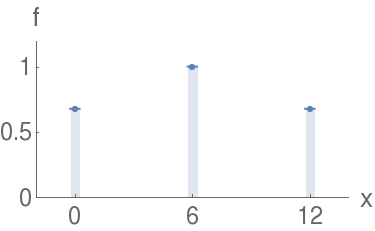
\includegraphics[width=0.94\textwidth]{Slike/discreteExample}
        \vspace{0mm}
        \caption{}
    \end{subfigure}
    \hspace{0mm}
    \begin{subfigure}[b]{0.32\textwidth}
        \centering
        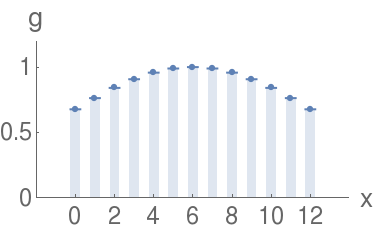
\includegraphics[width=0.94\textwidth]{Slike/discreteExample2}
        \caption{}
    \end{subfigure}
    \hspace{0mm}
    \begin{subfigure}[b]{0.32\textwidth}
      \centering
      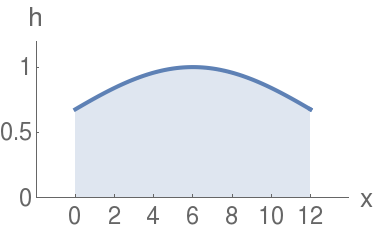
\includegraphics[width=0.94\textwidth]{Slike/discreteExample3}
      \caption{}
  \end{subfigure}
    \caption{Funkcije, ki živijo v (a) 3D, (b) 13D in (c) $\infty$-D funkcijskem (vektorskem) prostoru.}
    \label{fig:discreteExample}
\end{figure}

Na dimenzije vektorja gledamo kot na \textbf{prostostne stopnje}, katerih vrednosti lahko poljubno nastavljamo. Funkcijo $f$ (slika \ref{fig:discreteExample}a) zapišemo s komponentami in baznimi vektorji kot:
\begin{equation}
   \ket{f} =
   \begin{pmatrix}
      \mkern1mu 0,68 & 1,00, & 0,68 \mkern1mu
   \end{pmatrix}
   \begin{pmatrix}
      \mkern1mu \delta(x) \\
      \delta(x-6) \\
      \delta(x-12) \mkern1mu
   \end{pmatrix}
   =
   \mkern2mu 0,68 \, \delta(x) + 1,00 \, \delta(x-6) + 0,68 \, \delta(x-12)
   \ ,
   \label{eq:discreteF}
\end{equation}
Funkcijo $g$ (slika \ref{fig:discreteExample}b) zapišemo s komponentami in baznimi vektorji kot:
\begin{equation}
   \ket{g} =
   \begin{pmatrix}
      \mkern1mu 0,68 & 0,76 & \cdots & 0,68 \mkern1mu
   \end{pmatrix}
   \begin{pmatrix}
      \delta(x) \\
      \delta(x-1) \\
      \vdots \\
      \delta(x-12)
   \end{pmatrix}
   =
   \mkern2mu 0,68 \, \delta(x) + 0,76 \, \delta(x-1) + ... + 0,68 \, \delta(x-12)
   \ .
   \label{eq:discreteG}
\end{equation}
Še vedno veljajo vsa pravila vektorskih prostorov. Tako je na primer skalarni produkt funkcije $\ket{f}$ same s seboj enak:
\begin{equation}
   \bra{f}\ket{f} =
   \begin{pmatrix}
      \mkern1mu 0,68 & 1,00, & 0,68 \mkern1mu
   \end{pmatrix}
   \begin{pmatrix}
      0,68 \\
      1,00 \\
      0,68
   \end{pmatrix}
   =
   1,92 \ .
\end{equation}
Skalarni produkt je definiran le za funkciji znotraj istega funkcijskega prostora. Pri zvezni funkciji $h$ (slika \ref{fig:discreteExample}c) komponent in baznih vektorjev ne moremo našteti, ker jih je neštevno neskončno. Kljub temu lahko funkcijski vektor izrazimo analogno, kot smo to storili v diskretnih primerih \eqref{eq:discreteF} in \eqref{eq:discreteG}. Diskretno vsoto členov pretvorimo v zvezno vsoto (integral):
\begin{equation}
   \ket{h} = \int_{0}^{12} h(x_0) \mkern3mu \delta(x-x_0) \mkern5mu \text{d}x_0 = h(x) \text{ na območju } x \in [0, 12] \ .
\end{equation}
Skalarni produkt dveh zveznih funkcij je po analogiji enak:
\begin{equation}
   \bra{h}\ket{h} =
   \int_0^{12} h(x) \mkern2mu h(x) \mkern5mu \text{d}x \ .
\end{equation}
Če skalarne funkcije predstavimo kot funkcijske vektorje, kako potem na isti način predstavimo vektorske funkcije (ki slikajo v več skalarnih spremenljivk)? Tako, da vsako komponento (skalarno funkcijo) posebej zapišemo kot funkcijski vektor. Tako dobimo vektor vektorjev, oz. matriko. Zdaj vidimo, zakaj smo temelje \texttt{FEM} opisali brez uporabe omenjenih konceptov. Zahtevnost zapisov enačb se zmanjša na račun povečane zahteve po predstavljivosti zapisov. Kot primer v novem jeziku zapišimo variacijsko izjavo \eqref{eq:LsfemVariationalStatement}:
\begin{equation}
		\bra{\mkern1mu \mathbsf{A} \! \cdot \! \mathbf{v} \mkern2mu}\ket{\mkern2mu \mathbsf{A} \! \cdot \! \mathbf{u} - \mathbf{f}\mkern1mu} \ = \,
		0 \ , \hspace{5mm} \forall \mathbf{v} \ .
	\label{eq:LsfemVariationalStatementNew}
\end{equation}
To izgleda veliko bolje, kajne?

Za numerično reševanje problema moramo abs\-trakt\-no zastavitev \eqref{eq:LsfemVariationalStatement} z neskončno prostostnimi stop\-nja\-mi diskretizirati. Iskanje želimo omejiti na $N$ čim enakomerneje razporejenih točk, ki jih imenujemo \textbf{vozlišča}. V vsako vozlišče postavimo \textbf{vozliščno bazno funkcijo}, ki pokrije le okolico vozlišča:
\begin{IEEEeqnarray*}{rc}
    \hspace{16mm} \ket{\Phi_i} \, , \hspace{5mm} i = 1, ..., N \hspace{16mm} & \texttt{vozliščne funkcije .}
\end{IEEEeqnarray*}
Neskončno število neskončno ozkih stolpičev smo zamenjali s končnim številom ($N$) končno ozkih grbin. Problemu omejimo število prostostnih stopenj tako, da dopustimo le obstoj tistih funkcij $v(\mathbf{x})$, ki so superpozicija vozliščnih funkcij. To so funkcije, ki jih lahko zapišemo kot vrsto vozliščnih funkcij $\Phi_i(\mathbf{x})$ s koeficienti $v_i$:
\vspace{-3mm}
\begin{equation}
    \ket{v} = \sum_{i = 1}^N v_i \ket{\Phi_i} \ .
    \label{eq:nodalSeries}
\end{equation}
S tem problem prevedemo na iskanje $N$ \textbf{vozliščnih vrednosti} $v_i$. Naslikajmo idejo na skrajno preprosti kvadratni domeni $[-3,\mkern2mu 3\mkern1mu] \mkern-1mu \times \mkern-1mu [-3,\mkern2mu 3\mkern1mu]$ s krajevnim vektorjem $\bm{\chi} = \{\xi,\eta\}$. Nanjo postavimo pravokotno mrežo s šestnajstimi vozlišči (slika \ref{fig:regionAndNodeFunctions}a) in nad njimi napnemo prav toliko vozliščnih funkcij z nastavljivimi višinami $v_i\mkern1mu$ (slika \ref{fig:regionAndNodeFunctions}b).

\begin{figure}[ht]
   \centering
    \begin{subfigure}[b]{0.42\textwidth}
        \centering
        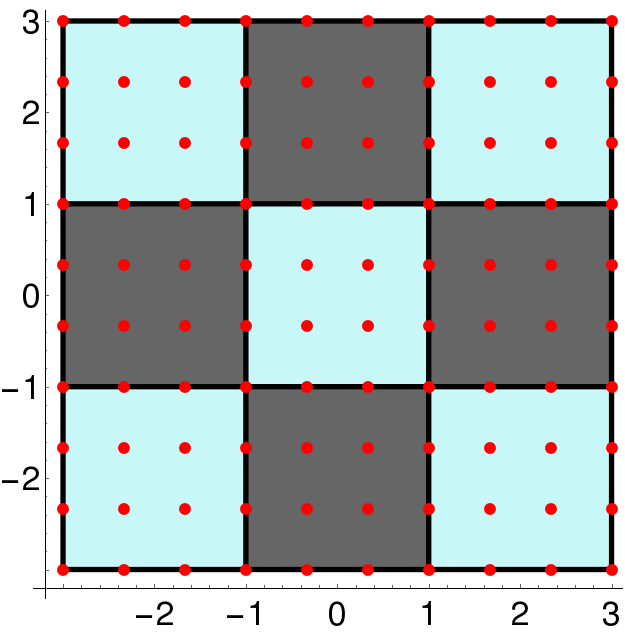
\includegraphics[width=0.94\textwidth]{Slike/layout2d}
        \vspace{0mm}
        \caption{}
    \end{subfigure}
    \hspace{5mm}
    \begin{subfigure}[b]{0.42\textwidth}
        \centering
        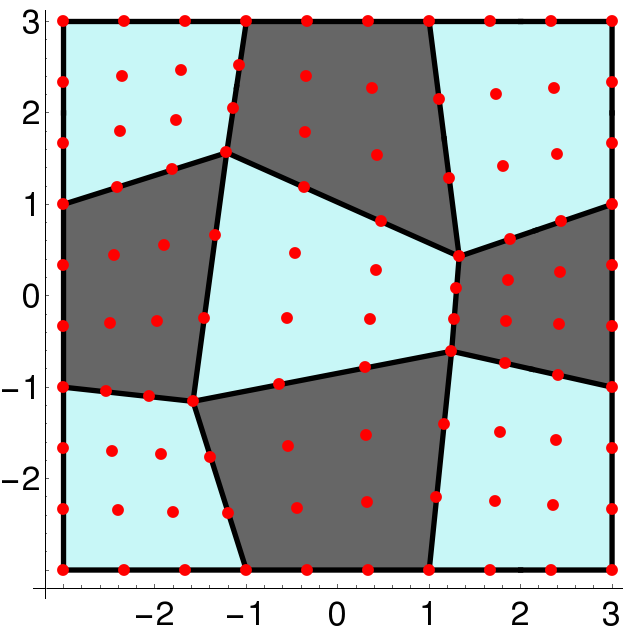
\includegraphics[width=0.94\textwidth]{Slike/layout2dTrans}
        \caption{}
    \end{subfigure}
    \caption{(a) Pravokotna domena z devetimi elementi (modre številke) in šestnajstimi vozlišči (rdeče številke) ter (b) nad vozlišči napete vozliščne funkcije. V prid nazornosti rišemo le štiri osrednje vozliščne funkcije.}
    \label{fig:regionAndNodeFunctions}
\end{figure}

\begin{figure}[ht]
   \centering
    \begin{subfigure}[b]{0.48\textwidth}
        \centering
        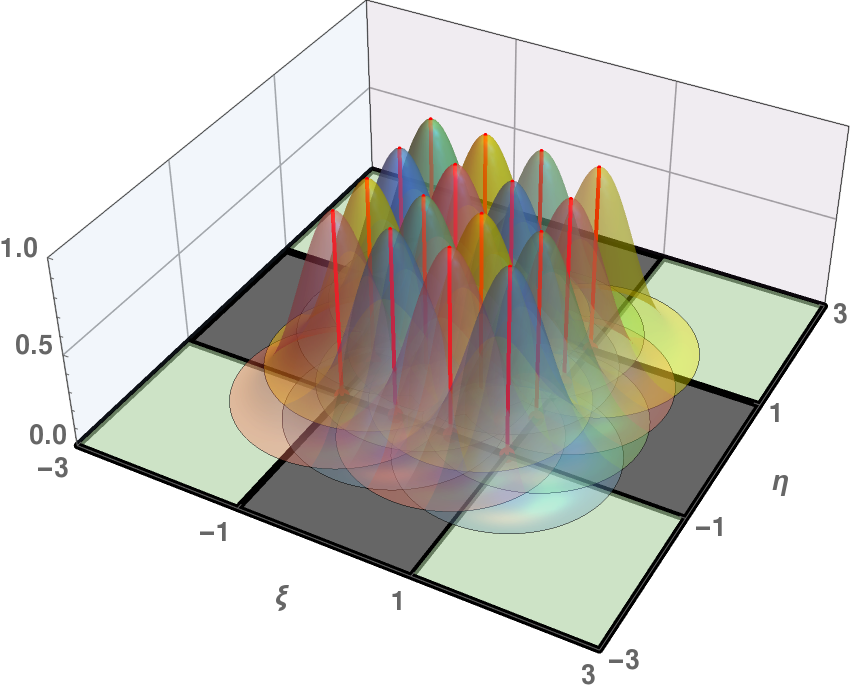
\includegraphics[width=0.94\textwidth]{Slike/nodalFuncs3d}
        \vspace{0mm}
        \caption{}
    \end{subfigure}
    \begin{subfigure}[b]{0.46\textwidth}
        \centering
        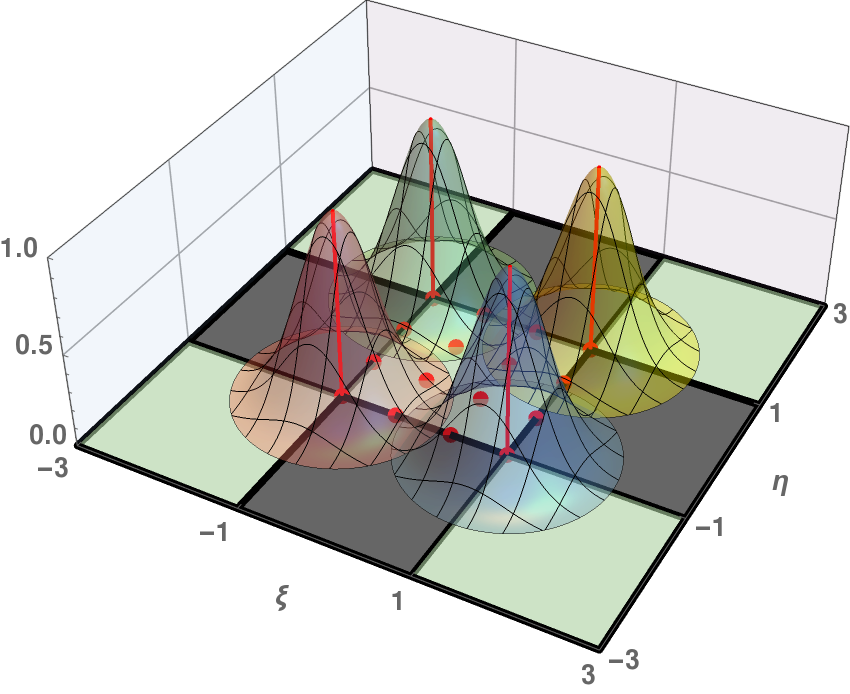
\includegraphics[width=0.94\textwidth]{Slike/nodalFuncs3dSparse}
        \caption{}
    \end{subfigure}
    \caption{}
    \label{fig:shapeFs}
\end{figure}

Štirikotne ploskvice, ki nastanejo s postavitvijo vozlišč, imenujemo \textbf{elementi}. Nobena vozliščna funkcija $\Phi_i$ ne sme pokrivati elementov, ki niso v stiku z njenim vozliščem. S tem dosežemo, da je $v(\bm\chi)$ nad nekim elementom sestavljena le iz funkcij v neposredni bližini tega elementa. Tako je $\mathbf{v}(\bm\chi)$ na sliki \ref{fig:sumAndShapeFunctions}a nad osrednjim elementom popolnoma določena z vrednostmi $v_6, v_7, v_{10}$ in $v_{11}$.

Ozrimo se na variacijsko izjavo \eqref{eq:LsfemVariationalStatement} ter si predstavljajmo funkcije $\mathbsf{A}(\mathbf{x}), \mathbf{u(x)}, \mathbf{v(x)}$ in $\mathbf{f(x)}$ zapisane v smislu razvoja po vozliščnih funkcijah \eqref{eq:nodalSeries}. Zaslutimo, da bomo računali prekrivne integrale vozliščnih funkcij:
\begin{equation}
    \bra{\Phi_i}\ket{\Phi_j} \ .
\end{equation}
To je enostavno dokler so vsi elementi iste oblike in velikosti, kot na sliki \ref{fig:regionAndNodeFunctions}. Takrat je dovolj, da izračunamo prekrivne integrale za vozlišča enega elementa. Kaj pa, če želimo uporabljati elemente poljubne oblike? Kako naj čim učinkoviteje, če so elementi poljubne oblike

 Segmente vozliščnih funkcij $\Phi_6, \, \Phi_7, \, \Phi_{10}$ in $\Phi_{11}$, ki se nahajajo neposredno nad elementom 5, proglasimo za \textbf{elementarne funkcije} $\phi_{5 j}(\bm\chi)$ tega elementa (slika \ref{fig:sumAndShapeFunctions}b). Tako lahko funkcijo $\mathbf{v}$ na

\begin{figure}[ht]
   \centering
    \begin{subfigure}[b]{0.48\textwidth}
        \centering
        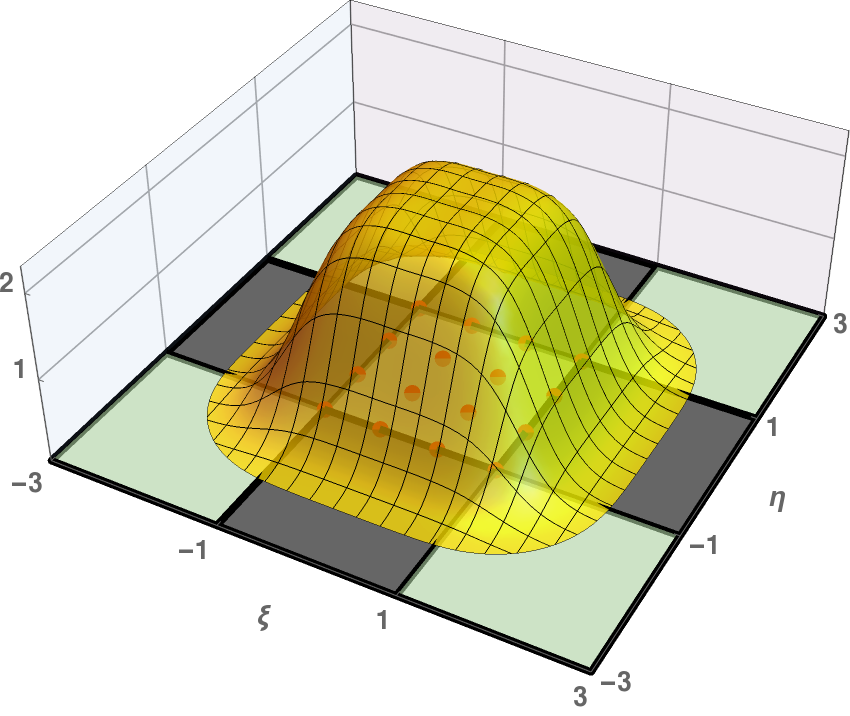
\includegraphics[width=0.94\textwidth]{Slike/nodalFuncsSumOverElm}
        \vspace{0mm}
        \caption{}
    \end{subfigure}
    \begin{subfigure}[b]{0.48\textwidth}
        \centering
        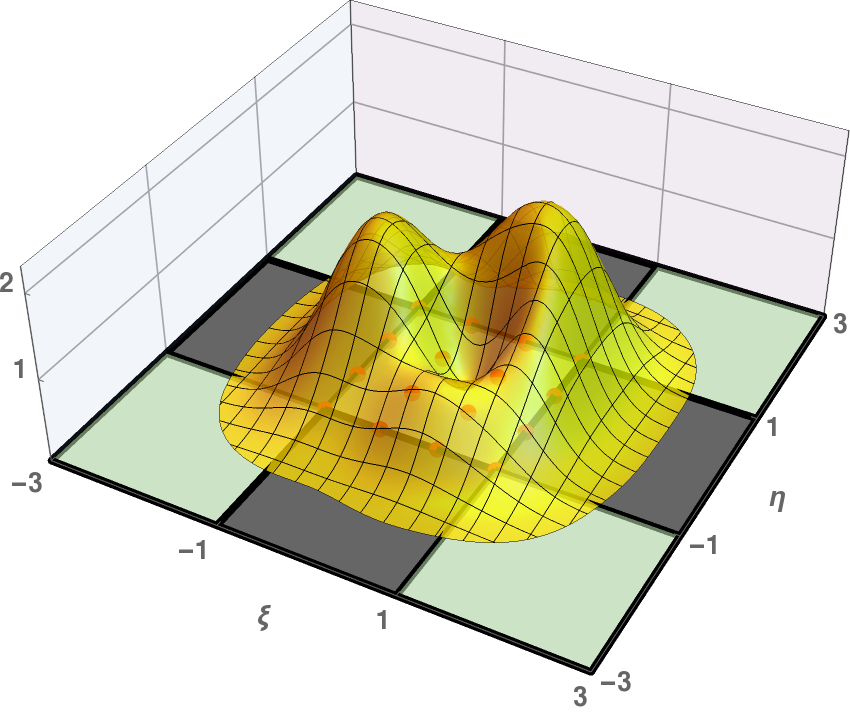
\includegraphics[width=0.94\textwidth]{Slike/nodalFuncsSumOverElmMod}
        \caption{}
    \end{subfigure}
    \caption{(a) vsota vozliščnih funkcij s slike \ref{fig:regionAndNodeFunctions}b in (b) elementarne funkcije, ki pripadajo elementu 5.}
    \label{fig:sumAndShapeFunctions}
\end{figure}

\begin{figure}[ht]
   \centering
   \begin{subfigure}[b]{0.44\textwidth}
       \centering
       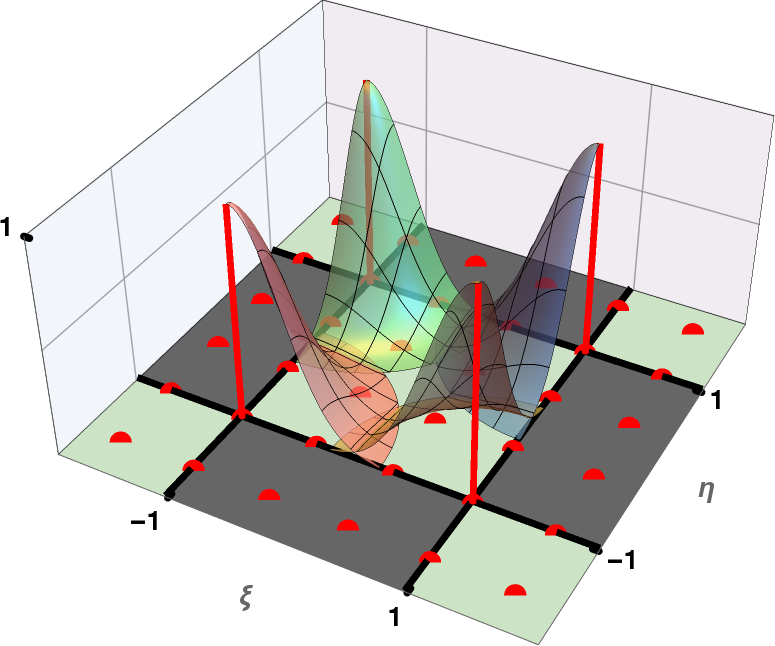
\includegraphics[width=0.94\textwidth]{Slike/elmFuncs3d}
       \vspace{0mm}
       \caption{}
   \end{subfigure}
   \hspace{3mm}
   \begin{subfigure}[b]{0.45\textwidth}
       \centering
       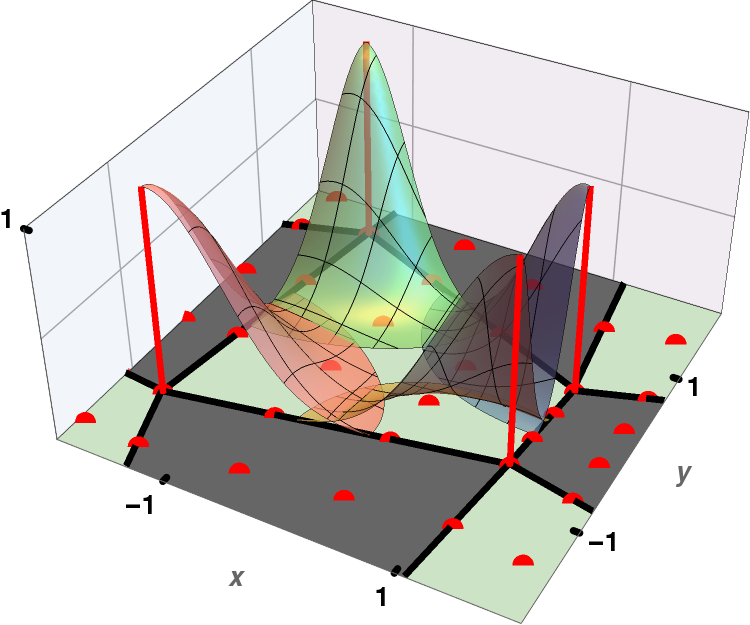
\includegraphics[width=0.94\textwidth]{Slike/elmFuncs3dTrans}
       \caption{}
   \end{subfigure}
   \caption{}
   \label{fig:shapeFs}
\end{figure}

še vedno  Z natančno analitično izpeljavo se prebijemo do izjave \eqref{eq:LsfemVariationalStatement}, od tod dalje pa moramo iskanje funkcije $\mathbf{u(x)}$ z neskončno prostostnimi stopnjami poenostaviti v iskanje funkcije s končnim številom prostostnih stopenj $N$. 

Skozi oči \texttt{FI} je $\ket{\Phi_i}$ eden izmed baznih vektorjev v razvoju vektorja $\ket{v}$, $v_i$ pa pripadajoča komponenta.
V jeziku funkcionalne analize (\texttt{FI}) pravimo, da smo omejili funkcijski prostor.

nadaljujemo z diskretizacijo problema, to je, pretvorbo na sistem $N$ algebrajskih enačb. Ta korak je enak pri vseh različicah \texttt{FEM}. Funkcije na domeni $\Omega$ imajo neskončno štveilo prostostnih stopenj. 
\begin{equation}
    u_i(\mathbf{x}) = \sum_{a = 1}^N \Phi^{a0} u^{a0}_i
\end{equation}

Mreža je v tem šolskem primeru strukturirana, kar pomeni, da je razporeditev elementov Kartezična. Mreža je lahko pri \texttt{FEM} tudi nestrukturirana, kar je ena izmed prednosti metode.

Potem omejimo Diskretizacija problema 

Galerkin, Najmanših kvadratov \cite{JiangB-LSFEM}
Basic lemma of variational principles: Temeljni lema variacijskih načel.


\begin{equation}
   \sum_i \bra{\left(A^{ab}_{jk} \mkern1mu \phi^{a0} \frac{\pd}{\pd x_b}\right) \left(v^c_k \mkern1mu \phi^{c0}\right)}\ket{\left(A^{de}_{jm} \mkern1mu \phi^{d0} \frac{\pd}{\pd x_c}\right) \left(u^g_m \mkern1mu \phi^{g0}\right) - f^h \mkern1mu \phi^{h0}}
\end{equation}

\begin{equation}
   \sum_i \bra{A^{ab}_{jk} v^c_k \phi^{a0} \phi^{cb}}\ket{A^{de}_{jm} u^g_m \phi^{d0} \phi^{ge} - f^h_j \phi^{h0}}
\end{equation}

\begin{equation}
   \sum_i v^c_k \left( \mkern2mu A^{ab}_{jk} A^{de}_{jm} u^g_m \bra{\phi^{a0} \phi^{cb} \mkern1mu}\ket{\mkern1mu \phi^{d0} \phi^{ge}} - \mkern1mu A^{ab}_{jk} \mkern1mu f^h_j \bra{\phi^{a0} \phi^{cb} \mkern1mu}\ket{\mkern1mu \phi^{h0}} \mkern2mu \right) = 0
\end{equation}
	\appendix
	\printbibliography
\end{document}
